\subsubsubsubsection{Roadway stretch}
\begin{figure}[h]
\centering
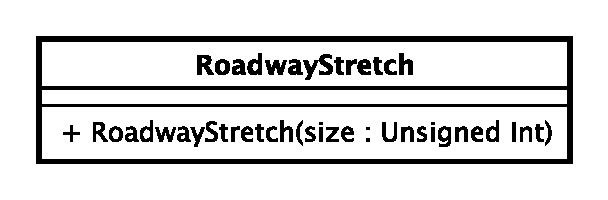
\includegraphics[scale=0.6,keepaspectratio]{images/solution/app/backend/roadway_stretch.eps}
\caption{\pReactiveComponentStretch::RoadwayStretch}
\label{fig:sd-app-roadway_stretch}
\end{figure}
\FloatBarrier
\begin{itemize}
  \item \textbf{\descr} \\
    It represents a roadway stretch entity. It is a protected object. All
    vehicles but bikes can tread this kind of stretch.
    \item \textbf{\ops}
  \begin{itemize}
    \item[+] \texttt{RoadwayStretch(size : Unsigned Int)} \\
        Creates a roadway stretch object with a specific size.
  \end{itemize}
\end{itemize}
